% This is samplepaper.tex, a sample chapter demonstrating the
% LLNCS macro package for Springer Computer Science proceedings;
% Version 2.20 of 2017/10/04
%
\documentclass[runningheads]{llncs}
%
\usepackage{graphicx}
\usepackage[utf8]{inputenc} % allow utf-8 input
\usepackage[T1]{fontenc}    % use 8-bit T1 fonts
\usepackage{hyperref}       % hyperlinks
\usepackage{url}            % simple URL typesetting
\usepackage{booktabs}       % professional-quality tables
\usepackage{amsfonts}       % blackboard math symbols
\usepackage{nicefrac}       % compact symbols for 1/2, etc.
\usepackage{microtype}      % microtypography
\usepackage{lipsum}
\usepackage{subfig}
\usepackage[a4paper,margin=1.5in,footskip=0.25in]{geometry}

% Used for displaying a sample figure. If possible, figure files should
% be included in EPS format.
%
% If you use the hyperref package, please uncomment the following line
% to display URLs in blue roman font according to Springer's eBook style:
% \renewcommand\UrlFont{\color{blue}\rmfamily}

\begin{document}
%
\title{Which book is the right one for me? \newline  Predicting tones of a book using its reviews}
%
%\titlerunning{Abbreviated paper title}
% If the paper title is too long for the running head, you can set
% an abbreviated paper title here
%
\author{Jiaming Qu. Ximing Wen, Wan Zhang, Jiesong He}
%
\authorrunning{J. Qu et al.}
\institute{University of North Carolina at Chapel Hill \\ Chapel Hill, NC \\}
%
\maketitle              % typeset the header of the contributionS
%

\section{Introduction}

NoveList is a provider of research databases, e-books and discovery service to libraries of all kinds, which is established by UNC alumni. It defines the different aspects of a book that may catch readers’ attention ``story elements''. The story elements include appeal terms, themes, and genres. Appeal terms, which is referred to as ``tone'' in our project, are a signature feature of NoveList \footnote{https://www.ebscohost.com/novelist/idea-center/learn/learn-story-elements}. NoveList imagine them as the secret language of books, all the ways a book speaks to a reader and lingers long after it’s been returned to the library. And appeal terms help readers find exactly what kind of book they are in the mood for.\par

Currently librarians NoveList are tagging each book with appropriate tones manually, which is quite labor-intensive and time-consuming. Therefore, given a book, an algorithm which automatically predicts its tones would be much helpful. In this project, we are using reviews and genres of a book as its metadata, as we assume that these two fields have richer information than other fields like title and author. Since usually each book has more than one tones, our task becomes a multi-label classification problem.

\section{Dataset Overview}
The data for this project is provided by Novelist. This dataset consists of 28737 books yet not all the books have review and tone fields. For prediction, We use a subset with 7005 books having reviews recorded and tones labeled. Our analysis of the dataset reveals that the 59 tones are not evenly distributed. As is shown in Fig ~\ref{fig1}, top 3 most frequent tones used are ``suspenseful'' (12.1\%), ``atmospheric'' (7.6\%), and ``moving'' (6.8\%). While the 3 tones being mentioned least are ``sad'' (0.1\%), ``liberal'' (0.1\%), and ``patriotic'' which is only for 3 books. On average, each book has 1.5 tones and each tone is assigned to 180 books.

\begin{figure}[!bh]
  \centering
  \begin{minipage}[b]{0.49\textwidth}
    \includegraphics[width=\textwidth]{s1.eps}
    \caption{Tone Distribution}
    \label{fig1}
  \end{minipage}
  \hfill
  \begin{minipage}[b]{0.49\textwidth}
    \includegraphics[width=\textwidth]{s2.eps}
    \caption{Review Distribution}
    \label{fig2}
  \end{minipage}
\end{figure}

Besides, each book has 1.5 reviews on average. Fig ~\ref{fig2} shows that 86.3\% books have 1 to 3 reviews. Almost 15.4\% books are given 4 reviews. But the percentage drops dramatically when referring to books with 5 and 6 reviews. There are only 73 and 2 books receiving 5 and 6 reviews respectively.

\section{Methodology}
In this section, we show in detail how we build the model to predict tones of a book using its reviews. We first provide the preliminary knowledge of multi-label classification which is the foundation of our proposed model. Then we give a heuristic approach as our baseline, followed by two machine learning approaches, namely the \emph{book-level} and \emph{review-level} respectively.

\subsection{Multi-label Classification}
Multi-label classification is different from multi-class classification. Multi-class classification implies that the amount of unique labels is at least 2, and when the amount is exactly 2, it is binary classification. However, multi-label classification emphasizes that each instance has at least one label and some instances may have more than one. In this project, we are dealing with both multi-class (59 uniques tones) and multi-label (each book has 1.5 tones on average) classification.

There are a lot of methods which transform the multi-label classification problem to a simpler form. Binary Relevance (BR) proposes it could be $L$ separate binary problems with one for each label, in which $L$ is the amount of labels \cite{luaces2012binary}. Then $L$ one-vs-all classifiers could be trained. But BR does not model label dependency, as some labels could be correlated instead of independent. Label Powerset (LP) proposes it could be a single multi-class problem with $2^{L}$ possible class values, and any multi-class classifier could be trained \cite{tsoumakas2010random}. But LP introduces too many class labels and much complexity. Pairwise Binary (PW) proposes it could be $L* \frac{(L-1)}{2}$ binary classifiers, which is known as all-vs-all \cite{petrovskiy2006paired}. Then each model is trained based on examples annotated by at least one of the labels, but not both. But the number of classifiers could be very high. Apart from these basic transformations, there are some advanced methods like classifier chains \cite{read2009classifier}, ensemble \cite{read2008multi} and etc. In this project, we use the BR method and we train 59 classifiers for 59 tones.

\subsection{Heuristic Approach}
Before we dive into machine learning techniques to tackle this problem, we start from a heuristic approach first. Since the two most frequent tones in the corpus are ``suspenseful'' and ``atmospheric'', we do a majority guessing which assumes that all the books only have these two tones. This approach gives us an interpretable lower bound when the learning process is purely based on counting.

\subsection{Machine Learning Approach}
It is a common practice to use machine learning techniques to deal with text classification problems. As is discussed above, the Binary Relevance transformation is used, therefore we need to train 59 binary classifiers for all the tones, and the Logistic Regression model is used for binary classification. These independent classifiers predict how much likely an instance has such a tone.

In terms of feature selection, we first only use text features which are unigrams after text pre-processing including converting to lower case, removing punctuations, removing stop words and stemming. We then add genres as a high-level feature into the model.

\textbf{Book-level Approach} As is shown in the dataset overview section, there are a lot of books with more than 1 reviews, and on average each book has 1.5 reviews. To deal with this issue, we first simply concatenate all the reviews for each book, then we predict its tones based on the merged review. Despite the simplicity and convenience, some books may have an extremely long review after concatenating, thus the features could be very sparse in the bag-of-words model.

\textbf{Review-level Approach} An alternative approach is to predict tones of a book based on all its reviews, and we train binary classifiers using all the reviews as the corpus, which means we predict tones from reviews. As is shown in Fig ~\ref{fig3}, instead of directly predicting labels, for each book we first split its reviews and then use each piece of review to predict the probabilities of tones. Then we take the average of these probability vectors as the probabilities of tones assigned to the book. Since each book has 1.5 tones on average, we then sort the probability from high to low and select two tones with the highest probability as the predicted label.

\begin{figure}
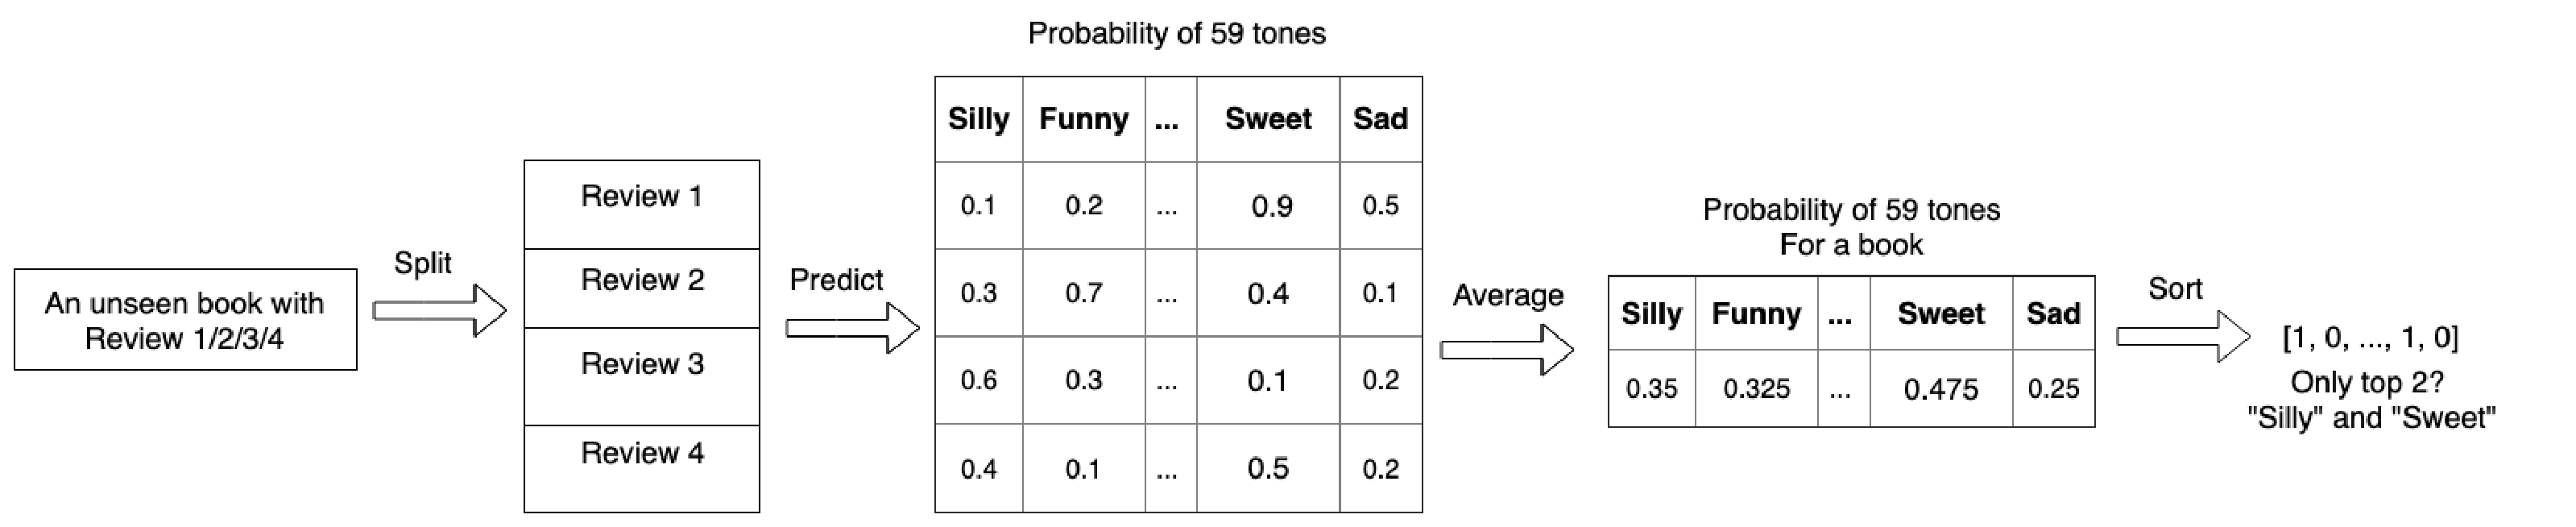
\includegraphics[width=\textwidth]{s3.eps}
\caption{Work flow of our proposed model} 
\label{fig3}
\end{figure}

\section{Result and Comparison}

We first use \emph{Hamming Loss} which is calculated as:
\begin{equation}
\frac{1}{NL} * \sum _{i=1}^{N} \sum _{i=1}^{L} I [\hat{y}^{(i)}_{j} \ne y^{(i)}_{j}]
\end{equation}

\noindent and \emph{Zero-one Loss} which is calculated as:
\begin{equation}
\frac{1}{N} * \sum _{i=1}^{N} I [\hat{y}^{(i)} \ne y^{(i)}]
\end{equation}

\noindent to compare the heuristic approach and machine learning approach, in which $L$ is the number of labels and $N$ is the number of instances, and $I[c]$ returns 1 if condition $c$ holds. \emph{Hamming Loss} could be understood as how many mistakes the prediction for an instance makes for each label, while \emph{Zero-one Loss} consider all the labels, i.e., predictions for all the labels should be exactly the same with true labels. 

\begin{table}[!htb]
 \caption{Comparison of Hamming Loss and Zero-one Loss}
  \centering
  \begin{tabular}{llll}
    \toprule
     & \textbf{Heuristic Approach} & \textbf{Book-level} & \textbf{Review-level} \\
    \textbf{Hamming Loss} & 0.0495 & \textbf{0.026} & 0.040\\
    \textbf{Zero-one Loss} & 0.983 & 0.995 & \textbf{0.966}\\
    \bottomrule
  \end{tabular}
  \label{compare}
\end{table}

\begin{figure}[!htb]
\includegraphics[width=\textwidth]{s4.eps}
\caption{Comparison of Average Precision and Recall @K} 
\label{fig4}
\end{figure}

Table ~\ref{compare} summarizes performances of the three approaches mentioned above. It is surprising that concatenating all the reviews for a book outperforms splitting reviews. However, as we pry into the result, we found that most labels predicted by the book-level approach are all 0, and since there are a few 1's in the true labels, its \emph{Hamming Loss} is much more lower. These two metrics are too vague and hard to interpret. Therefore, we change these two evaluation metrics to another two metrics which are more interpretable. In real work, librarians who use the model may care about not only what the predicted labels are, but also what are the most possible ones. Thus, instead of predicting labels, we predict probabilities of 59 tones, sort from high to low, and return a ranked list of 59 tones, which is transformed into a ranking problem. We use Precision and Recall @K to evaluate how these approaches perform. 

As is shown in Fig ~\ref{fig4}, the review-level approach which predicts on reviews and then take the average has a significant improvement over the book-level approach which predicts on all the reviews of a book. Also, adding genres as high-level features further enhances this approach.

\section{Conclusions}
In this project, we use reviews and genres of a book to predict its tones. The feature of a book is represented in TF-IDF vectors from text and count vectors from genres, and 59 Logistic Regression models are trained. The results prove that splitting reviews, predicting probabilities and taking average outperforms concatenating reviews, and adding genres as a high-level feature further improves the performance.

\section{Acknowledgement}
We appreciate Novelist for sharing the data and Dr. Yue Wang from the School of Information and Library Science for supervising the whole project. 

\newpage
\bibliographystyle{unsrt}
\bibliography{references.bib}
\end{document}
